\documentclass{article} % For LaTeX2e
\usepackage{nips13submit_e}
\usepackage{hyperref}
\usepackage{url}
%\documentstyle[nips13submit_09,times,art10]{article} % For LaTeX 2.09
\usepackage{pifont}
\usepackage{times,amsmath,color, balance,tabularx,caption,
amssymb,graphicx,epsfig,cite,psfrag,subfigure,multirow,cases,algorithmic,mathtools}
\usepackage{longtable}
\usepackage{booktabs}
\usepackage{adjustbox}
\usepackage[ruled,vlined]{algorithm2e}

\newtheorem{claim}{Claim}
\newtheorem{guess}{Conjecture}
\newtheorem{definition}{Definition}
\newtheorem{fact}{Fact}
\newtheorem{assumption}{\underline{Assumption}}
\newtheorem{theorem}{\underline{Theorem}}
\newtheorem{lemma}{\underline{Lemma}}
\newtheorem{ctheorem}{Corrected Theorem}
\newtheorem{corollary}{\underline{Corollary}}
\newtheorem{proposition}{Proposition}
\newtheorem{example}{\underline{Example}}
\newtheorem{remark}{\underline{Remark}}
\newtheorem{problem}{\underline{Problem}}
\def\Ei{\mathop\mathrm{Ei}}
\def\E{\mathop\mathrm{E}}
\def\tr{\mathop\mathrm{tr}}
\newcounter{mytempeqncnt}

\title{Decoding Team Composition in MOBA Games \\ A Learning Approach}


\author{
Jiachen Li$^*$, Yilin He$^\dag$, and Chengliang Lian$^*$\\
Language Technologies Institute$^*$ and Machine Learning Department$^\dag$ \\ School of Computer Science \\
Carnegie Mellon University, Pittsburgh, PA, 15213 \\
\texttt{\{jiachenl, yilinhe, clian\}@andrew.cmu.edu}
}

% The \author macro works with any number of authors. There are two commands
% used to separate the names and addresses of multiple authors: \And and \AND.
%
% Using \And between authors leaves it to \LaTeX{} to determine where to break
% the lines. Using \AND forces a linebreak at that point. So, if \LaTeX{}
% puts 3 of 4 authors names on the first line, and the last on the second
% line, try using \AND instead of \And before the third author name.

\newcommand{\fix}{\marginpar{FIX}}
\newcommand{\new}{\marginpar{NEW}}

\nipsfinalcopy % Uncomment for camera-ready version

\begin{document}


\maketitle

\begin{abstract}
Team composition of massive online battle arena (MOBA) games has become an interesting as well as challenging problem studied by many researchers and companies. In the setting of MOBA games, a good team compositions will improve the chance of winning, while a bad team compositions might ruin your game.
In this project, we applied machine learning method to analyze the impact of team composition on the MOBA game results. We collected data from two most popular MOBA games: DotA 2 and LoL. We proposed two feature models in representation of data and compared algorithms with different characteristics such as Logistic Regression (LR), Support Vector Machine (SVM) and Deep Belief Networks (DBN), which are used to train the predicting model. Our experiments proved that the team composition could, to some degree, predict the winning of games and we gave further analyses to the intrinsic relationship of the results.
\end{abstract}

\section{Introduction}


%\begin{center}
%   \url{http://papers.nips.cc}
%\end{center}


Multiplayer online battle arena (MOBA) is a rising force in faced-paced and single-round online games that also involves team play. In the past few months, more than 27 million players played against each other per day in one of such kind of game called League of Legends (LoL) [1] while millions are attracted by another game called Defense of the Ancient 2 (DotA2). International MOBA tournaments are held over the world with a prize pool of over \$10 million [2].  Analysis on MOBA games will not only gain us experience of data analysis but also be beneficial to players and game companies all over the world.

In MOBA games like LoL or DotA 2, two groups of five players are pitted against each other based on their levels of game proficiency. In the beginning of a game, each player first picks an unique character out of over 100 options, and then the five characters controlled by a group of players form a team in the game. There are many common strategies for picking characters that can yield a good team composition. As the game begins, players control selected characters to battle for victory. A typical game would last 30--60 minutes.

There are many factors that influence end game results. Player's proficiency, team composition, and in-game strategy are some important aspects of MOBA game play. Although intuitively individual player's proficiency might sounds like the biggest factor of their chance of winning, it is not true because the game system is designed to select players with similar proficiency in a match. As a result, team composition and in-game strategy plays a much more important role in determining the game outcome.

In this project, we are interested in analyzing the impact of team composition on game outcome. Strategies to form a good team composition to achieve highest winning probability is always a heated topic for the online communities as well as professional teams. The challenging part for this problem is the large number of possible team compositions. To be specific, since there are generally more than 100 characters for players
to choose, the number of possible team compositions for both teams are more than $\binom{100}{5}\cdot\binom{95}{5}\approx 4\times 10^{15}$.

To answer this question, we can transform it into a classification problem in machine learning: given a team composition, predict the result for the game. With this problem transformation, we can learn how to form a good team composition by interpreting the learning model parameters and then form good team composition in practice by using the learned model for prediction and recommendation.

The goal of this project is to achieve a reasonable high accuracy on the prediction (e.g., more than 60\%). The prediction accuracy is limited by the nature of this problem. Achieving over 80\% accuracy implies that most of the game are determined in the character picking stage, which mean the following 30-60 minutes of actual game play have very little influence on the result. This is undesirable for the player. Therefore despite the fact that team composition is an important factor for end game result, our prediction accuracy shouldn't be too high.



%\subsection{Related Work}
%Conley and Perry have previously worked on predicting win ratio based on heroes picked by the team in DotA 2. In their work, they have reported 69\% accuracy using logistic regression and K-NN.

%\subsection{Organization of this Report}
%The remaining of this report is organized as follows: Section II presents the collection of the data set, Section III introduces the learning model and assumptions ..



\section{Data Set Preparation}
We have obtained two data sets for this study, one from the LoL and the other from DotA 2. The whole dataset contains more than 80,000 independent game history records in total, which are adequate for this project.

\subsection{Data Collection}

The dataset was collected through public APIs provided by the video game producers Riot and Steam, respectively. The APIs provide us a given number of most recent completed games as well as the corresponding statistics. To make full use of the APIs, we ran our feature collection program on AWS Cloud Computing platform to collect these data in a $7\times24$ manner.


\subsection{Data Contents}

The contents of the original data collected from APIs are shown as follow:


\begin{itemize}
\item \textit{Game Id}: an Unique identifier for the game, used to avoid data redundancy;
\item \textit{Game duration}: duration of each game, used for data cleaning;
\item \textit{Winner}: the winning team, used as labels;
\item \textit{Team composition}: the characters selected by each team, used as the main features;
\item \textit{Skill levels}: the players' performance in their history, used to evaluate the potential performance of the players;
\item \textit{KDA Statistics}: the character's performance in this game, i.e., number of other characters it killed (K), number of times it died (D), and numberof times it assisted its teammate to kill the other characters (A).
\end{itemize}

\subsection{Data Cleaning}

As we all known that the performance of machine learning algorithms is heavily dependent on the quality of features. So before extracting features from raw data, we need to do some data cleaning.

Since the public APIs always return the most recent game records, we should first to check whether there is any redundancy in our data set. Besides, we need to make sure the data is useful, which can be verified from the game duration. For example, if the game duration is too short, then it is likely that some player leaves the game early and causes imbalanced performance. In this case, the record may not be able to support our learning goal and should be discarded. Finally, we will have a look at the KDA statistics, if some character's KDA is below a normal level, then this character may not fully participate into the game. Therefore, the corresponding record should also be dropped.

After finishing these procedures, we can then extract features from the data and train our models.


\section{Models and Assumptions}

In this section, we proposed two models for decoding team composition. ``Character Ranking Model'' analyzes the team composition by ranking the importance of each character in the team, and ``Predicting Model with Prior'' takes the characters' prior knowledge such as the player skill level and the winning probability between different characters into consideration. The first model can be used to interpret the parameters while the second model is mainly used to improve the predicting performance.

\begin{figure}[t]
  \centering
    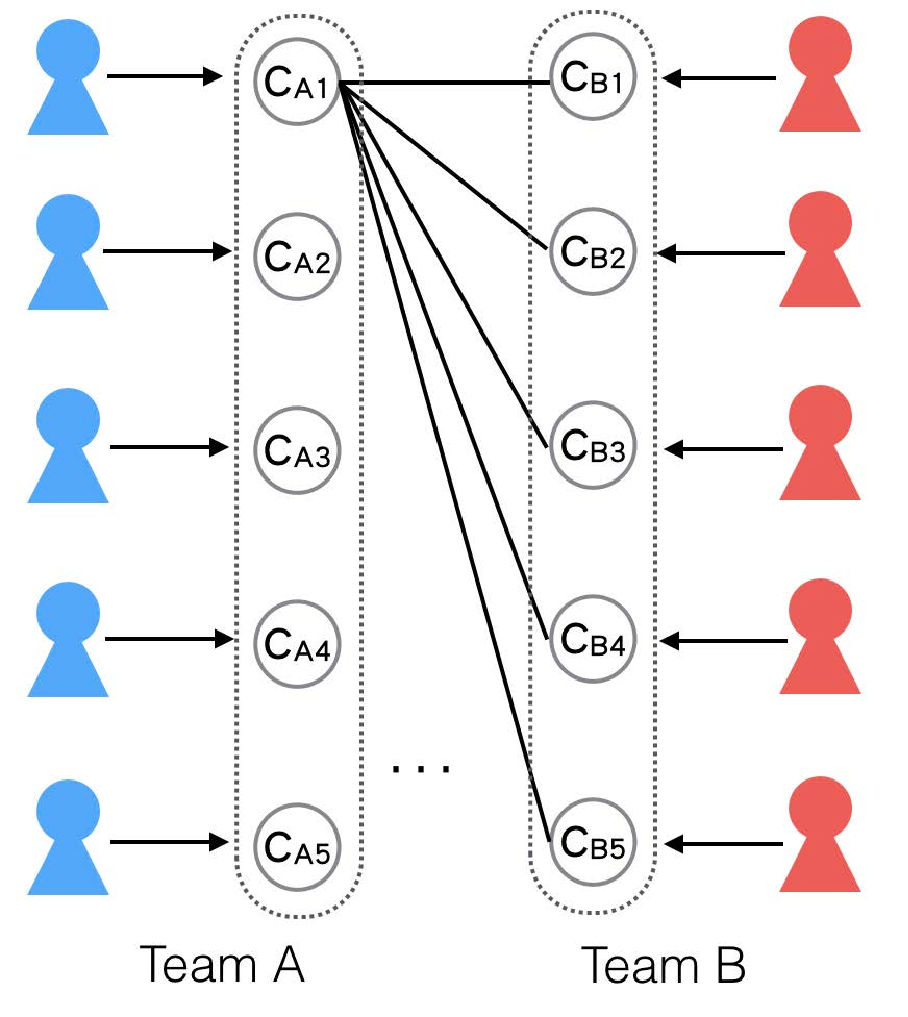
\includegraphics[width=60mm]{team_comp.pdf}
  \caption{An illustration of team composition and the aspects that may influences the game result.}
  \label{fig:team_comp}
\end{figure}



To start discussing the models,  as shown in Fig. \ref{fig:team_comp}, let's first define the two teams in the game as team $\mathcal{A}$ and team $\mathcal{B}$, where each team contains five unique characters (i.e., $c_{A1},\ldots,c_{A5}$ for team $\mathcal{A}$ and $c_{B1},\ldots,c_{B5}$ for team $\mathcal{B}$). Moreover, suppose that the game has $N$ different characters in total, then all the characters can be encoded with an integer from $1$ to $N$.

\subsection{Model-I: Character Ranking Model}

In the character ranking model, the characters in each team are encoded as some kind of indicator vector, and what we really want to learn from this model is the corresponding weights for different characters in the machine learning algorithms, especially the one from a linear decision boundary, which measures how important the character to a team. To introduce the that, we may first need to make some assumptions:

\begin{assumption}
We assume that players in both team all have high skills. And they are proficient with the characters they pick.
\end{assumption}

\begin{remark}
This assumption is reasonable because we only collected the records of players with
higher skill levels during the data collection part. Moreover, in order to win the game, the players are not likely to pick the characters that they are not familiar with.
\end{remark}

With this assumption, we can further assume that the game result is independent of the players, then we can use the vector $\textbf{x}=\{x_1,x_2,\ldots,x_N\}$ to represent the training feature. The element $x_i$ indicates the presence of $i$-th character in the game, and the value is given by

\begin{equation}
x_i =
\begin{cases}
1 &  \text{if $i\in \mathcal{A},$} \\
-1 &  \text{if $i\in \mathcal{B},$} \\
0 & \text{otherwise.}
\end{cases}
\end{equation}

Besides, the team that wins the game will serve as the label for the corresponding feature.


\subsection{Model-II: Predicting Model with Prior}


Unlike the character ranking model where we make independence assumptions between
player skills and game results. This predicting model takes the relationship of different characters into account, and let it work as the prior information. For example, Fig. \ref{fig:team_comp} has shown the factors that may have potential influence on the game result. It can be seen from this figure that the performance of one specific character should have connections with all the other characters in the opposite team. This is not difficult to understand because there are many times in the game that all the characters in a team will need to work together to achieve their goals. Therefore, to learn the team composition, we also need such information.

To utilize these additional information, we first define the character matrix.
\begin{definition}
A matrix $C \in \mathbb{R}^{N\times N}$ is called the character matrix if the element $c_{i,j}$ indicates the probability that the team with character $i$ beats the team with character $j$, i.e. $c_{i,j}=\text{Pr}\{\text{team with character $i$ wins when played against team with $j$}\}$.
\end{definition}

The character matrix can be computed from the statistics of game history and it gives a character performance evaluation between different character pairs that can be used for learning. Based on that, we introduce the following model. For each team, we have two feature vectors. Let's take team $\mathcal{A}$ as an example, the feature vectors can be defined as:
\begin{equation}
\mathbf{a}=\{a_1,a_2,\ldots,a_N\} \ \ \ \ \ \ \ \ \ \ \ \ \ \ \ \
\mathbf{a'}=\{a_1',a_2',\ldots,a_N'\},
\end{equation}
where the elements are defined as:
\begin{equation}
a_i =
\begin{cases}
1 & \text{if $i\in\mathcal{A}$}\\
0 & \text{otherwise}
\end{cases}\ \ \ \ \
a_i' =
\begin{cases}
\prod_{j\in \mathcal{B}} c_{i,j} & \text{if $i\in\mathcal{A}$} \\
0 & \text{otherwise}
\end{cases}
\end{equation}

The feature vector $\mathbf{a}$ shows the characters chosen in team $\mathcal{A}$, while the feature vector $\mathbf{a'}$ indicates the ``likelihood'' that team $\mathcal{A}$ with character $c_{Ai}$ beats team $\mathcal{B}$, where the $c_{i,j}$ is the element from character matrix $C$.

After obtaining the similar two feature vectors for team $\mathcal{B}$ (i.e., $\mathbf{b}$ and $\mathbf{b'}$), we can then build the modified feature vector for this model, which is $\textbf{x}=\{\mathbf{a},\mathbf{a'},\mathbf{b},\mathbf{b'}\}$.

\begin{remark}
Note that in the midway report we proposed a feature matrix $F \in \mathbb{R}^{N\times N}$ and wanted to utilize players information (i.e., use a function $g(P_{\mathcal{A},i},P_{\mathcal{B},j})$ to evaluate the winning ratio between two players) to enhance the feature. The element of feature matrix $F$ is designed as
\begin{equation*}
f_{i,j}=c_{i,j} \cdot g(P_{\mathcal{A},i},P_{\mathcal{B},j}),
\end{equation*}
where the $c_{i,j}$ is the element from character matrix, $g(P_{\mathcal{A},i},P_{\mathcal{B},j})$ is the function that measure the winning ratio between the player in group $\mathcal{A}$ using character $i$ and the player in group $\mathcal{B}$ using character $j$.

However, our progress after midterm showed that this approach is not available. The main difficulty is to find a reasonable way to do dimensionality reduction. We have tried to use the characters' KDA statistics to cluster them into several groups with k-means algorithm, but the results suggest that the differences between each two groups are quite small, which means that characters don't have clear patterns over the KDA statistics. This is reasonable since the KDA statistics are greatly influenced by players' in-game performance, so that even for the same character, different players may lead to totally different KDA. Besides, due to the privacy policy, we are not able to get the skill levels for all the players, which makes the evaluation more difficult.
\end{remark}

Compared with the feature matrix idea, this feature model uses a more compact approach to utilize the prior knowledge (e.g. convert the character-character relationship to character-team relationship through the winning ``likelihood''). Though this may lose some information about the exact relationship between every two characters, the modified feature only has a dimension of $4\times N$, which is just four times larger than that of character ranking model, so it doesn't suffer from the high dimension problem and is eligible for training.


\section{Evaluation and Discussion}

In this section, we apply our feature models to different machine learning algorithms, train different learning models and use them to achieve our goals such as evaluation of convergence, parameters interpretation, game result prediction and character recommendation.

The feature using Character Ranking model in the experiments is denoted as ``w/o prior'' while the feature using Predicting Model with Prior is denoted as ``w/ prior''. In general, we used $80\%$ of the whole data set as the training data, and the other $20\%$ as the test data. The detailed algorithm parameters setting is introduced in Game Result Predicting part.

\subsection{Evaluation of Convergence}


\begin{figure}[t]
  \centering
    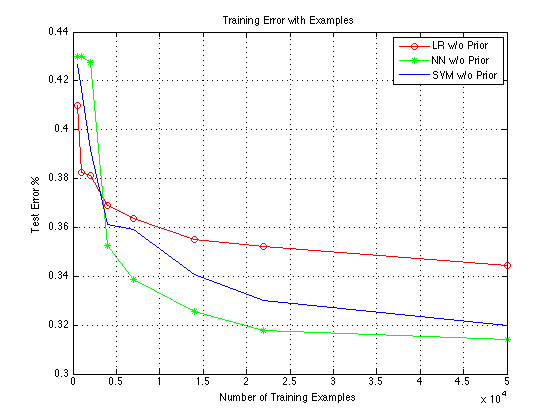
\includegraphics[width=90mm]{resWOprior.png}
  \caption{The test error versus number of training data for Character Ranking Model}
  \label{fig:2}
\end{figure}


\begin{figure}[t]
  \centering
    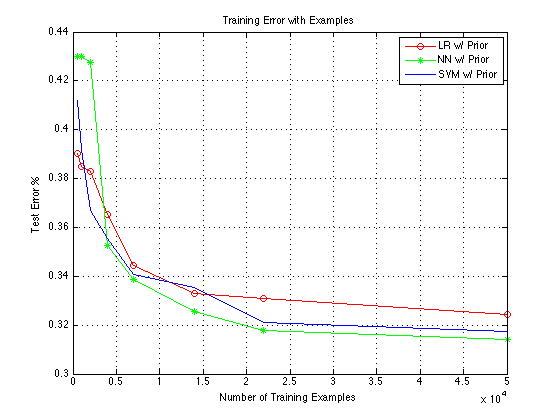
\includegraphics[width=90mm]{withPrior.png}
  \caption{The test error versus number of training data for Predicting Model with Prior}
  \label{fig:3}
\end{figure}

The first part of the evaluation is about the convergence of different algorithms over different training data size, which can be used to check whether our collected data sets are large enough for this learning task. Note that We mainly did this part on the DotA 2 data set since its size is much larger than LoL and should be enough for our analysis.

It can be seen from Fig. \ref{fig:2} and \ref{fig:3}, as we increase the training data, the error rate of different algorithms converge quickly at first and then become more stable when the number of training data is larger than $25,000$, which can be regarded as a threshold that determines whether the data size is able to make some meaningful results. Besides, comparing the results from Fig. \ref{fig:2} and \ref{fig:3}, we can see that the learned model with features contain prior knowledge converges better, which gives us a hint that our Predicting Model with Prior may have better predicting performance.




\subsection{Parameter Interpretation}



If we use the machine learning algorithms that have a linear decision boundary for classification (e.g., Logistic Regression and linear kernel SVM), the parameters (e.g., $\mathbf{\beta}$) of the learned linear decision boundary (e.g., $f(\mathbf{X}) = \mathbf{\beta}\cdot \mathbf{X}$) will have a direct meaning under the Character Ranking model, i.e. each weight we get for the corresponding character implies how this character could impact on the final games result. In other words, it means that how important this character for the team!

\begin{figure}[h]
  \centering
    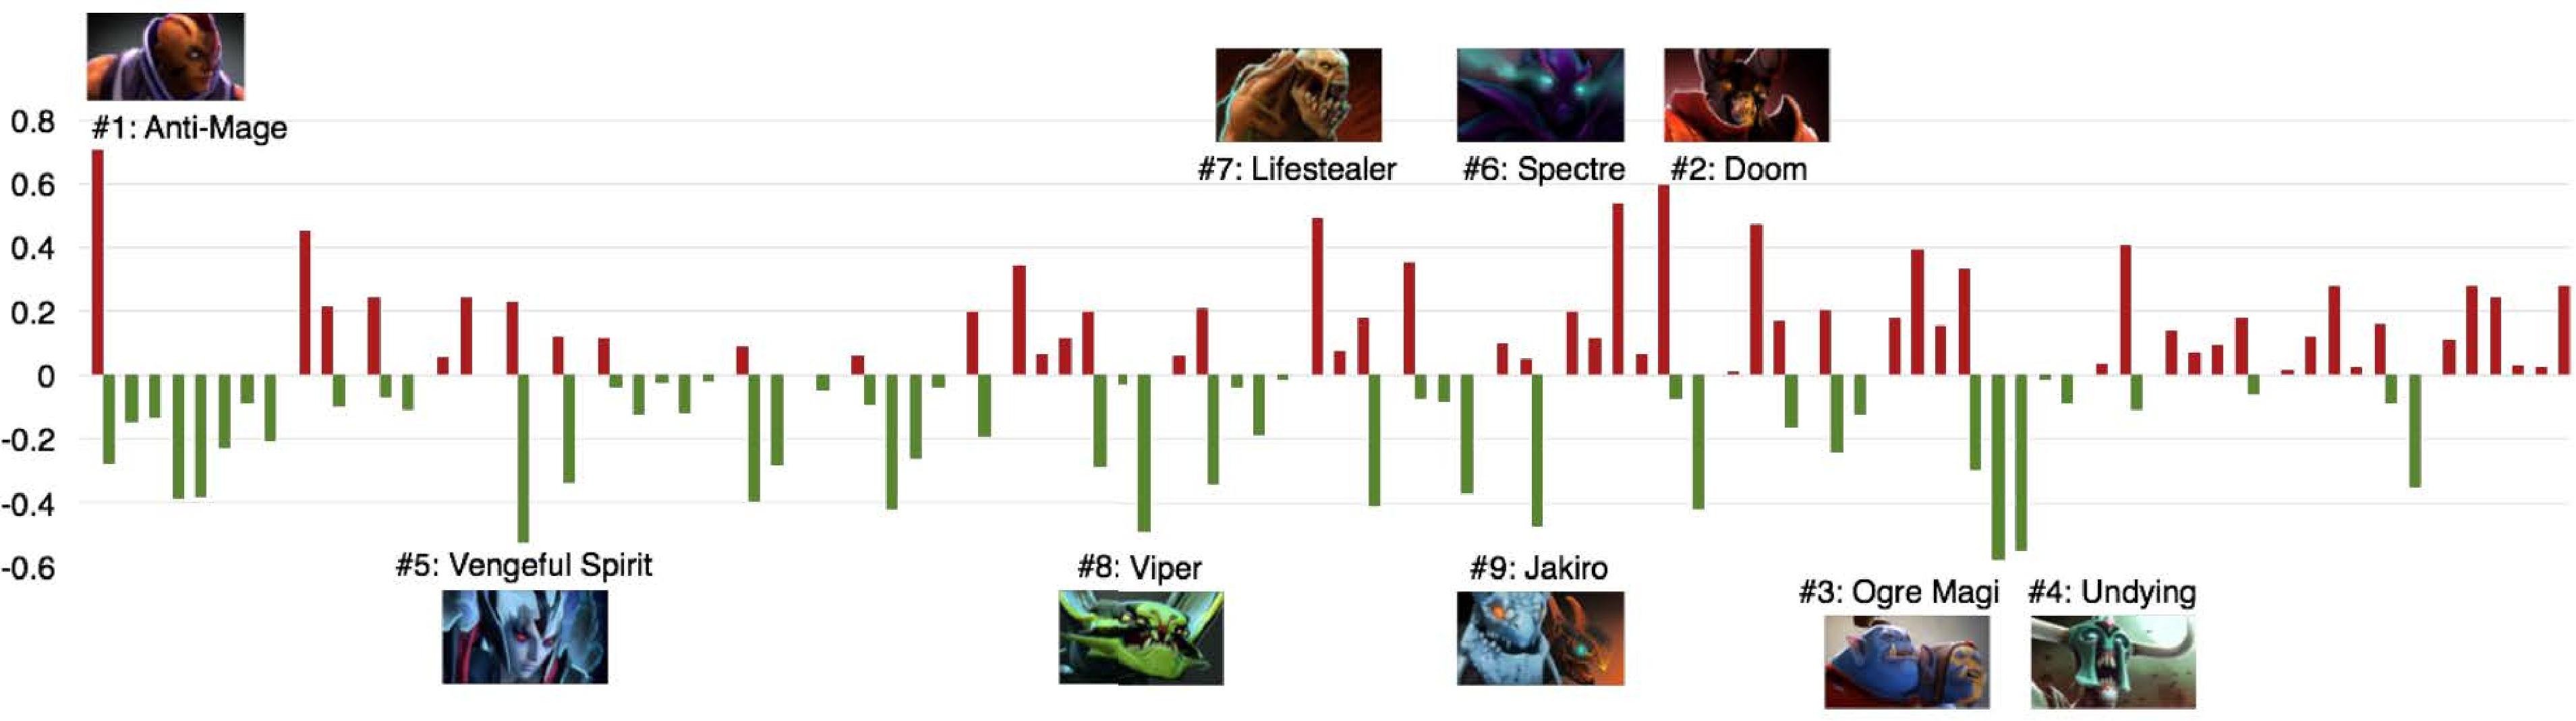
\includegraphics[width=125mm]{params.pdf}
  \caption{Visualization of linear model parameters using Character Ranking model.}
  \label{fig:params}
\end{figure}

Fig. \ref{fig:params} shows an example of parameters visualization from Logistic Regression using Character Ranking model. The weight vector we obtained can represent each character's influence on game result. For character $i$, a positive (red) weight means that picking this character will increase the chance of winning, while a negative (green) weight indicates that picking this character may decrease your chance for winning. Since we want to do prediction by ranking the importance of different characters, we do not consider synergy between characters. Therefore, during the prediction phase, given 2 teams that are comprised of different characters, we could expect the team with larger weights wins the game.

\begin{remark}
If you are familiar with DotA 2, you may find that the characters with high ranks are exactly the core players in the game based on players in-game experiences, which, from another perspective, shows that our learned ranking is reasonable and our feature model is correct.
\end{remark}




\subsection{Game Result Prediction}

\subsubsection{Parameters setting}

The logistic regression is implemented by maximizing the log-likelihood, the optimization algorithm used is gradient descent. The learning rate is set as 0.003 while the iteration times for each run is taken as 100.

The SVM is implemented based on the LIBSVM library [3]. We used soft-margin SVM and Gaussian Kernel for our classification problem, the cost $C$ is 1 and the $\gamma$ in radial basis function $\text{exp}(-\gamma \|u-v\|^2)$ is 0.07.

The Deep Belief Network (DBN) is implemented based on [4] and the DeepLearnToolBox developed by [5], we used a 3 hidden layers DBN with sigmoid unit, and the layer-wise dimensions are 108:54:54. The learning rate for neural network is taken as 0.001, the number of epochs for RBM pre-training is 10, and the number of epochs for fine-tuning is 100. The training strategy for DBN is batched gradient descent and output layer type is ``softmax''.

Note that this set of parameters are found by a combination of manually testing and cross validation.


\subsubsection{Results Analysis}

In this part, we analyze the prediction accuracy using our proposed feature models. The results reported in this part are the average value over multiple runs (we will shuffle the data in each run) with the parameters setting mentioned in the previous part.


\begin{table}[h]
\center
\captionsetup{font={small}}
\caption{Prediction result of different algorithms}
\begin{tabular}{|c |c |c |c |c |}
\hline
Algorithm & \multicolumn{2}{c|}{DotA 2}    & \multicolumn{2}{c|}{LoL}   \\
\hline
Accuracy (\%) & w/o prior   & w/ prior  & w/o prior  & w/ prior  \\ \hline
Logistic Regression    & 65.57         & 67.58     & 55.90         & 55.36
\\ \hline
SVM(Gaussian Kernel) & \textbf{68.02} & 68.24 & 55.97 & 56.45
\\ \hline
Deep Belief Networks  & 67.30  & \textbf{68.60}   & \textbf{56.10} & \textbf{56.80}     \\ \hline
\end{tabular}\label{tab:1}
\end{table}

It can be seen from the table that the prediction accuracies of SVM and DBN are very close, and they are also a little better than the result of LR. This is reasonable since SVM (with Gaussian kernel) and DBN are more complex model than LR (e.g., LR has a linear decision boundary while the other two have non-linear decision boundary), they should have the abilities to fit the data better.

For the Predicting model with Prior (e.g., w/o prior), its overall performance is better than the Character Ranking model, which means that the prior knowledge can help to improve the learning performance. Besides, we may also note that the prediction accuracy differences between two features for complex models are smaller than that for simpler model (i.e., Logistic Regression), which implies that this kind of prior is more useful for the simpler model.

Unlike using DBN for pattern recognition where we can interpret the neural network weights as learned patterns, we may not be able to directly interpret the parameters we obtained from neural networks here. Nevertheless, we can show some intuitive explanations for why Neural Network can learn a result that outperforms others. One the one hand, notice that the neural network contains a full connected architecture, and its learning process can capture the relationship between different characters from input layer and pass this relationship (by using weighted sum) to the next layer. On the other hand, we are using pre-training for the DBN, which is indeed an unsupervised feature learning process that can help DBN to initialize a set of good weights.

Finally, you may also be curious about why the prediction accuracy has great differences between these two data sets. According to our convergence analysis, the most possible reason is that the training data set for LoL is not as large as that of DotA 2 (i.e., we have 58000 valid records for DotA 2, but we only have 15000 valid records for LoL. This is because LoL's data is more difficult to collect than DotA 2). %To verify our guess, we also

\subsubsection{Advanced Discussion on Prediction Results}

Since our training feature is sort of sparse, we took Nicole's suggestion and added L1 penalty (Lasso) to the regression model. Moreover, we also took Prof. Gordon's suggestion by adding confidence interval on the results in this part of the study. Since SVM and DBN have already had the regularization, we only applied it to the logistic regression. Also, due to the limitation of time, we may not be able to compute the confidence intervals for all the machine learning model. So, we mainly focus on the logistic regression in this part and make some advanced discussions on the prediction results.

We ran L1-regularized and L2-regularized logistic regression on both data sets using R with LiblineaR package [6]. Besides, Package heuristicC was used to calculate cost parameter according to the Joachim's heuristics. In the pre-processing phase, our data were normalized by subtracting mean from each feature and dividing it by their standard deviation. The detailed results are shown in Table. \ref{tab:2}, where the confidence for the interval is of $95\%$.

\begin{table}[h]
\center
\captionsetup{font={small}}
\caption{Prediction results with confidence interval of regularized logistic regression}
\begin{tabular}{|c |c |c |c |c |}
\hline
Algorithm & \multicolumn{2}{c|}{DotA 2}    & \multicolumn{2}{c|}{LoL}   \\
\hline
Accuracy (\%)                       & w/o prior   & w/ prior  & w/o prior  & w/ prior  \\ \hline
LR + L1 penalty  & 67.70 $\pm$ 0.10    & 67.50 $\pm$ 0.11     & 56.30 $\pm$ 0.25  & 56.18 $\pm$ 0.25     \\ \hline
LR + L2 penalty   & 67.68 $\pm$ 0.12   & 67.44 $\pm$ 0.13  & 56.43 $\pm$ 0.22  & 55.18 $\pm$ 0.24 \\ \hline
\end{tabular} \label{tab:2}
\end{table}

According to the results, the confidence intervals are very small for all results in table 2, which indicates that our results are quite reliable. Moreover, we looked at the number of non-zero parameters in L1 regularized parameters and found out that over 90\% of the parameters are non-zero for Character Ranking model, which implies that only a small part of the feature makes no contribution, so most of the characters do have certain influence for the game results.

For the accuracies, it can be seen by comparing Table. \ref{tab:1} and Table. \ref{tab:2}. Both L1 and L2 regularization make the two models work better, which may due to penalty for some less meaningful parameters that is added by regularization.

\subsection{Character Recommendation}

In this part, we used our trained model to do character recommendation, which is also an useful application for our study.

In the MOBA games, the recommendation is usually in need at the following two situations:
\begin{itemize}
  \item When the opponents have finished team picking up, but your team still need another one character to pick. In this situation, we could consider picking any one of the characters left to form a team and use our trained model to compute the possibility of winning with this team.
  \item If both teams don't finish constructing, then we may apply the weights we learned from linear models to select the characters, as each weight reflects the overall chance of winning with this character.
\end{itemize}

A sample character recommendation algorithm is shown as follows. Note that the recommendation should not only consider the winning probability, but also consider the player's judgment. Therefore, it is more appropriate to return the top N (e.g., N=5) characters that have the high winning probability instead of just returning the character that have the highest winning probability.

\begin{algorithm}[h]
\KwIn{Characters Selected in Two Team $\mathcal{A}$ and $\mathcal{B}$; List of Characters $\mathcal{C}$}
\KwOut{list of the Recommended Character $X=\{x_1,x_2,\ldots,x_5\}$}
{\bf Procedure:} \\

{\bf If:} $|\mathcal{B}| = 5$  \\
	~~~~~ {\bf For} $x \in \mathcal{C} \backslash \{\mathcal{A,B}\}$\\
	~~~~~  ~~~~~ $Score(x) = h(\mathcal{A,B},x$) \\
	~~~~~ {\bf Return} top N $x$ of highest $Score(x)$ \\

{\bf Else:} \\
    ~~~~~ {\bf Return} top N $c \in \mathcal{C} \backslash \{\mathcal{A,B}\}$ with highest weights in the learned model.\\

\caption{{\bf Character Recommendation Algorithm} \label{Algorithm}}
\end{algorithm}




\section{Conclusions and Future Work}

\subsection{Conclusions}

In this project, we analyzed the team composition problem in MOBA games through a learning approach. We first proposed two feature models, and used them for training different machine learning models like LR, SVM and DBN. Furthermore, we added regularization and confidence intervals for part of the study, and provided more insights on the parameters as well as the reliability of the results. Experiment of the convergence analysis first demonstrated that our data set size was big enough to make meaningful results. The interpretation of parameters from linear decision boundary also indicated that our model did learn some meaningful results. We then showed in the results prediction part that the team composition did have connection with game results and the relationship is decodable. Finally, A character recommendation algorithm is built based on our learned results.


\subsection{Future Work}

The major limitation of our proposed feature models is that it only captures the team-level composition but doesn't capture some deep compositions like the different combinations of characters' specially abilities (e.g., like their unique skills). Therefore, we can explain which character is important for a team but we cannot explain in detail which factor of this character is the most important part for a good team composition. One way to solve this problem may be to add the details of each character's information into the feature, but this will make the feature too complex (high dimension) and hard to fit in the algorithms.

Nevertheless, this leads to some future works for dimensionality reduction of the features. A possible direction is by clustering different characters to several in-game roles by their specific abilities and skills. Usually in MOBA games, characters are designed to belong to one or more roles such as supportive or aggressive characters. Therefore if we are able to identify the role of each character in the team, we can reduce our dimension to a lower order of magnitude. Compared to cluster over KDA statistics, clustering based on characters' own attributes should be more reasonable and more reliable, and it is quite possible that it may lead to a better result.

\subsubsection*{Acknowledgments}

We authors would like to thank Nicole for her feedbacks as well as comments, which keep this projet on the right direction, and her suggestion of applying Lasso, which improves our predicting results. Moreover, we would also like to thank Prof. Gordon for his suggestion of adding the confidence interval to show the reliability of the results.

In addition, we also gave our great thanks to Steam and Riot for sharing game history data from public API.

\subsubsection*{References}
\small{

[1] Ian Sherr, ``Player Tally for League of Legends Surges,'' \textit{Digits RSS. N.p., n.d. Web}. 28 Sept, 2014.

[2] Valve, Dota 2 -- 2014 Compendium -- The International. Dota 2 Official Website.

[3] Chih-Chung Chang and Chih-Jen Lin, LIBSVM : a library for support vector machines. \textit{ACM Transactions on Intelligent Systems and Technology}, 2:27:1--27:27, 2011. Software available at
\url{http://www.csie.ntu.edu.tw/~cjlin/libsvm}.

[4] G. E. Hinton, S. Osindero, and Y. Teh, ``A fast learning algorithm for deep belief nets,'' \textit{Neural Computation}, 18, pp 1527--1554, 2006.

[5] R. B. Palm, Prediction as a candidate for learning deep hierarchical models of data, \textit{Master's thesis}, Technical University of Denmark (DTU), Informatics, 2012.


[6] R.-E. Fan, K.-W. Chang, C.-J. Hsieh, X.-R. Wang, and C.-J. Lin. LIBLINEAR: A Library for Large Linear Classification, \textit{Journal of Machine Learning Research} 9(2008), 1871-1874. Software available at \url{http://www.csie.ntu.edu.tw/~cjlin/liblinear}.

\end{document}
